\begin{figure}[ht]
	\capstart
	\centering
	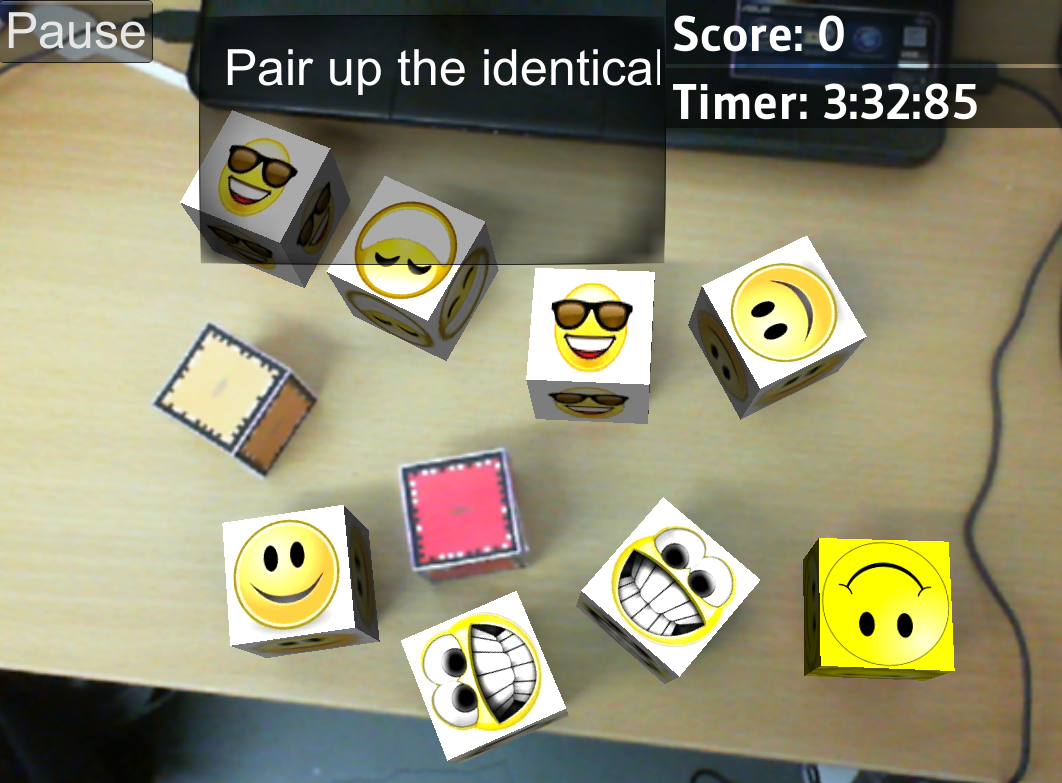
\includegraphics[width=0.8\textwidth]{images/MatchCubes}
	\caption{Match Cubes minigame}
	\label{fig:match_cubes}
\end{figure}


\subsection{Program flow chart}

\begin{figure}[ht]
	\capstart
	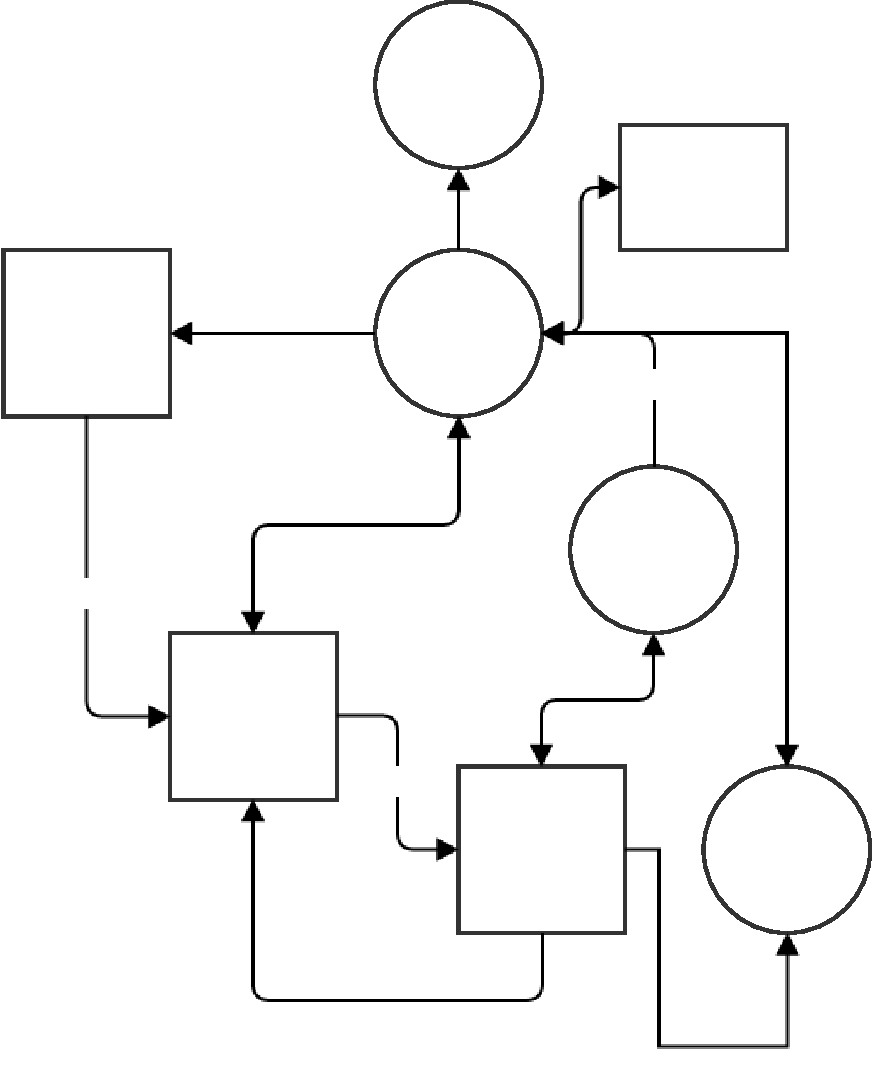
\includegraphics[width=\textwidth]{images/user_flow_chart}
	\caption[Program flow chart]{How a user maneuvers in the program.}
	\label{fig:program_flow_chart}
\end{figure}

Upon starting the program the user is presented with the main menu.
The main menu consists of four sets of buttons.

One set is the buttons that each lead to a single mini-game. 
When clicked they will take the player to the loading screen of the appropriate mini-game where the player can read instructions for the game and see current high-scores for that game.
After clicking the play button the user is taken into the game where the user can either play the mini-game or press the pause button.
If the user presses the pause button a pause screen is shown with the options of resuming the game, restarting from level one or go back to the main menu.

After the mini-game is completed the user is taken back to the loading screen if there is more levels left of the mini-game, otherwise the high-score list is shown.
The high-score lets the user go back to the main menu.

Back in the main menu, if the user presses the button "Change username" the user will be presented with a input field where a name can be entered, upon submitting a name the user will be brought back to the main menu.

If the user presses the "quit" button the application exits.

The last button on the main menu is the "Play all games" button. When the user presses this button it will play all the available mini-games in sequential order.